\documentclass[class={IEEEtran}]{standalone}
\usepackage{tikz}

\pagestyle{empty}
\usetikzlibrary{shapes.geometric,shapes.arrows,positioning,calc,arrows.meta,math}

\tikzset{ARROW/.style={thick, -stealth}}
\tikzset{ORACLE/.style={rectangle, minimum width=13.5em, minimum height=15.5ex, draw, semithick, align=flush left, anchor=north east}}

\linespread{1.25}

\begin{document}
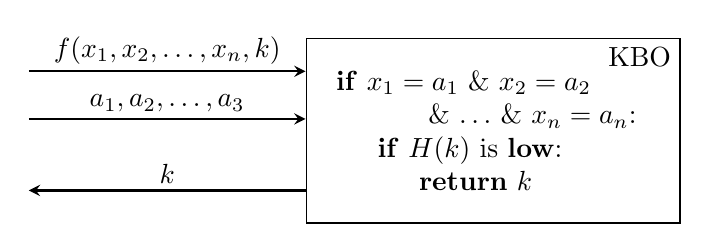
\begin{tikzpicture}
    \node[ORACLE] (n_oracle) {
        \hspace{-0.5em}\textbf{if} $x_1 = a_1$ \& $x_2 = a_2$ \\
        \hspace{2.5em} \& $ \ldots $ \& $ x_n = a_n $: \\
        \hspace{1.0em}\textbf{if} $H(k)$ is \textbf{low}:\\
        \hspace{2.5em}\textbf{return} $k$
    };
    \node[anchor=north east] at (n_oracle.north east) {KBO};

    \coordinate (input1) at ($(n_oracle.west)+(-10em, 5ex)$);
    \coordinate (input1_end) at ($(input1-|n_oracle.west)$);
    \draw[ARROW] (input1) -- (input1_end) node[midway,above=-0.3ex]{$f(x_1, x_2, \ldots, x_n, k)$};

    \coordinate (input2) at ($(n_oracle.west)+(-10em, 1ex)$);
    \coordinate (input2_end) at ($(input2-|n_oracle.west)$);
    \draw[ARROW] (input2) -- (input2_end) node[midway,above=-0.3ex]{$a_1, a_2, \ldots, a_3$};

    \coordinate (output) at ($(n_oracle.west)+(-10em, -5ex)$);
    \coordinate (output_end) at ($(output-|n_oracle.west)$);
    \draw[ARROW] (output_end) -- (output) node[midway,above=-0.3ex]{$k$};


\end{tikzpicture}

\end{document}
